\graphicspath{ {images/VM_Install} {images/Ubuntu_Intro} }

\chapter{Getting Started}
\label{chap:getting_started}

  As discussed in \autoref{sec:where_to_start} I strongly recommend using the provided
    Virtual Machine (VM) for this merit badges.
  Doing so allows for the following notable advantages:

  \begin{enumerate}
    \item Only one installation necessary
    \begin{itemize}
      \item All of the tools necessary for any project can be installed on the VM with one command
    \end{itemize}
    \item Guaranteed Compatibility
    \begin{itemize}
      \item All of the projects for this merit badge have been verified to work on the VM
    \end{itemize}
    \item Easier to Follow
    \begin{itemize}
      \item All of the instructions and examples in this project have been designed with the VM in mind
    \end{itemize}
    \item Improved Cyber Security
    \begin{itemize}
      \item Using a VM keeps all of the programming and activity which is done inside the VM separate from the main computer
    \end{itemize}
  \end{enumerate}

  The remainder of this chapter is spent allowing for install and a quick guide to the operating system.

  \section{Installing VM Software}
  \label{sec:installing_vm_software}

    There are a wide variety of VM software available on the market.
    I strongly recommend using Oracle's VirtualBox as it is free software which is created by a 
      reliable and trusted industry member.
    That being said if you prefer the use of a different VM software that should be easily supported
      by the rest of this project guide.

    \subsection{Installing VirtualBox}
    \label{ssec:installing_virtualbox}

      To start we need to download VirtualBox.
      This can be done by navigating to the official webpage at \href{https://www.virtualbox.org/wiki/Downloads}
        {https://www.virtualbox.org/wiki/Downloads} (see \autoref{fig:virtualbox_download_page}).
      Select the platform package which corresponds to the OS of your personal computer (macOS = OS X).
      
      \begin{figure}[ht]
        \centering
        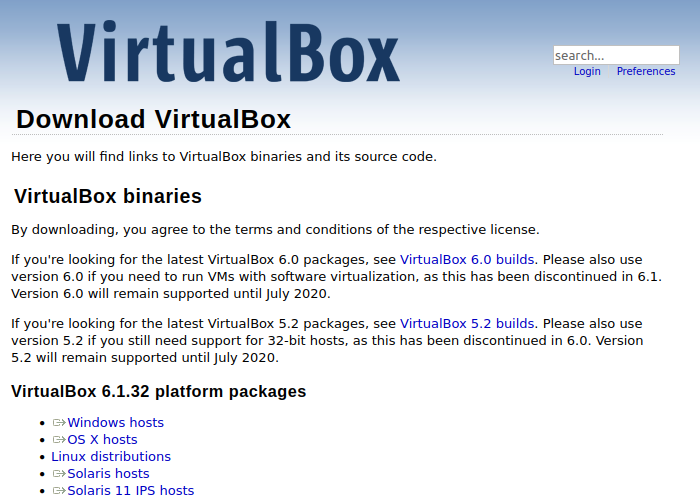
\includegraphics[width=0.8\linewidth]{virtualbox_download_page.png}
        \caption{VirtualBox Download Page}
        \label{fig:virtualbox_download_page}
      \end{figure}
      \FloatBarrier

      Run the executable and install VirtualBox by following the instructions.
      (\textit{Note: if prompted to choose which features are to be installed the following are required at a minimum; USB Support and Networking}).

  \section{Importing the Programming Merit Badge VM}
  \label{sec:import_merit_badge_vm}

    In order to provide the easiest starting spot for the VM a pre-made file has been created.
    Use a web-browser to navigate to the \href{Google Drive Folder}{https://drive.google.com/drive/folders/1rE8jUb4SAwdj-uCSRVqeH7lIxF3ttpCl?usp=sharing}
      and download the \texttt{Scouts\_Programming\_MB.ova} file.
    This is a fairly large file (it contains an entire computer after all) and may take awhile to download.
    (\textit{Note: if you are unable to download the file your councilor can provide you a USB drive which contains a copy of the file})

    Now open \texttt{VirtualBox} (installed \autoref{ssec:installing_virtualbox}).
    You should see a screen like shown in \autoref{fig:virtualbox_home_screen} at which point click the import arrow.
    This will open an import screen.
    Use this screen to select the \texttt{Scouts\_Programming\_MB.ova} we downloaded earlier and click \textit{next}.

    \begin{figure}[ht]
      \centering
      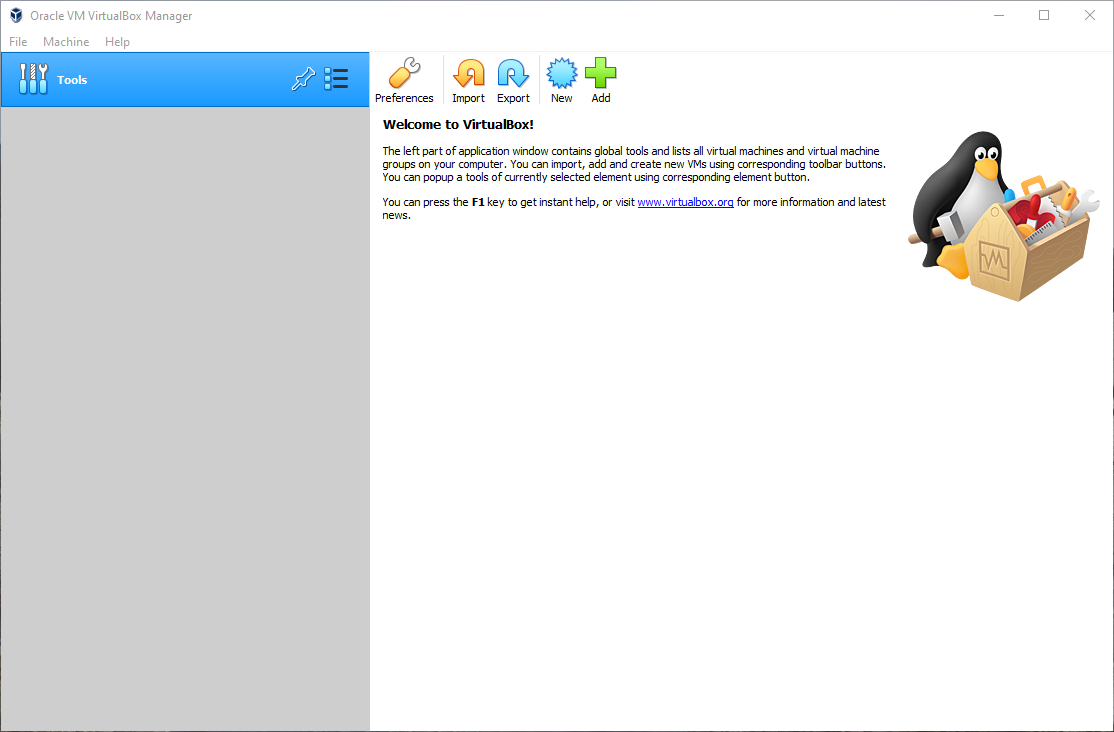
\includegraphics[width=0.8\linewidth]{virtualbox_home_screen.png}
      \caption{VirtualBox Home Screen}
      \label{fig:virtualbox_home_screen}
    \end{figure}
    \FloatBarrier

    This should bring up a screen like the one shown in \autoref{fig:virtualbox_advanced_mode}.
    Here you are able to set a lot of options about how you want your VM to behave.
    The two we are most interested in are \textit{CPU} and \textit{RAM}.
    If you know how many CPU cores or how much ram you have in your computer you can use up to half of each without having any issues.
    However, if you are unsure how your computer is equipped talk to your councilor or choose the safe \textit{CPU = 2} and \textit{RAM = 2048 MB}.

    \begin{figure}[ht]
      \centering
      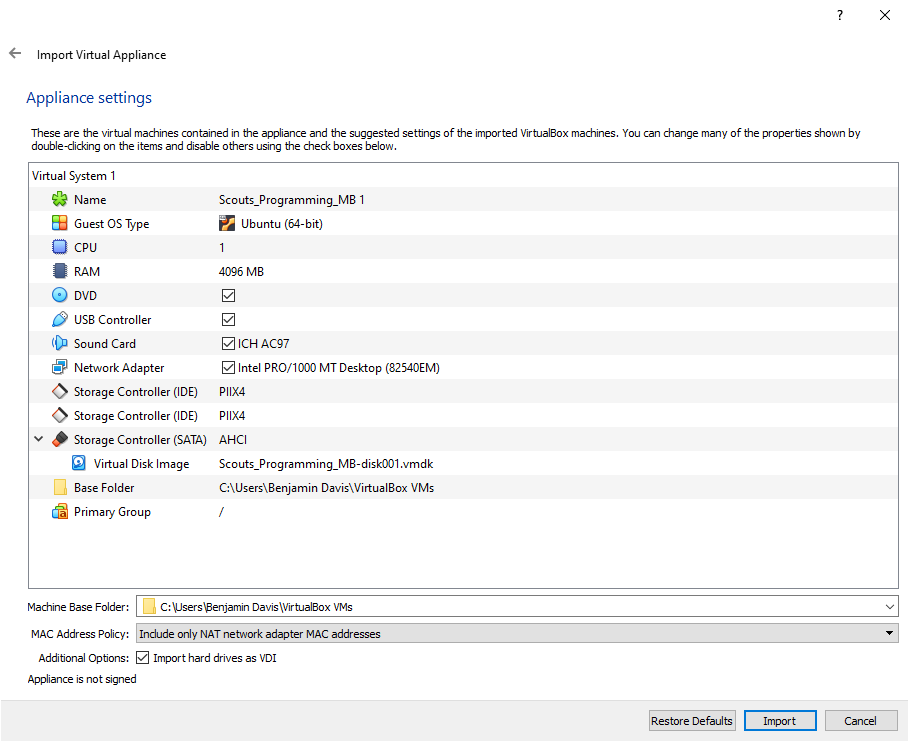
\includegraphics[width=0.8\linewidth]{virtualbox_advanced_mode.png}
      \caption{VirtualBox Advanced Settings}
      \label{fig:virtualbox_advanced_mode}
    \end{figure}
    \FloatBarrier

    Now hit import and wait a couple of minutes while the VM imports.
    Once the import is complete you should see the home screen again.
    This time there should be a Scouts\_Programming\_MB VM on the left side (as seen in \autoref{fig:virtualbox_import_complete}).
    Click this VM and then hit start.
    Now that you've got the VM imported head down to \autoref{sec:getting_familiar_with_vm} to continue!

    \begin{figure}[ht]
      \centering
      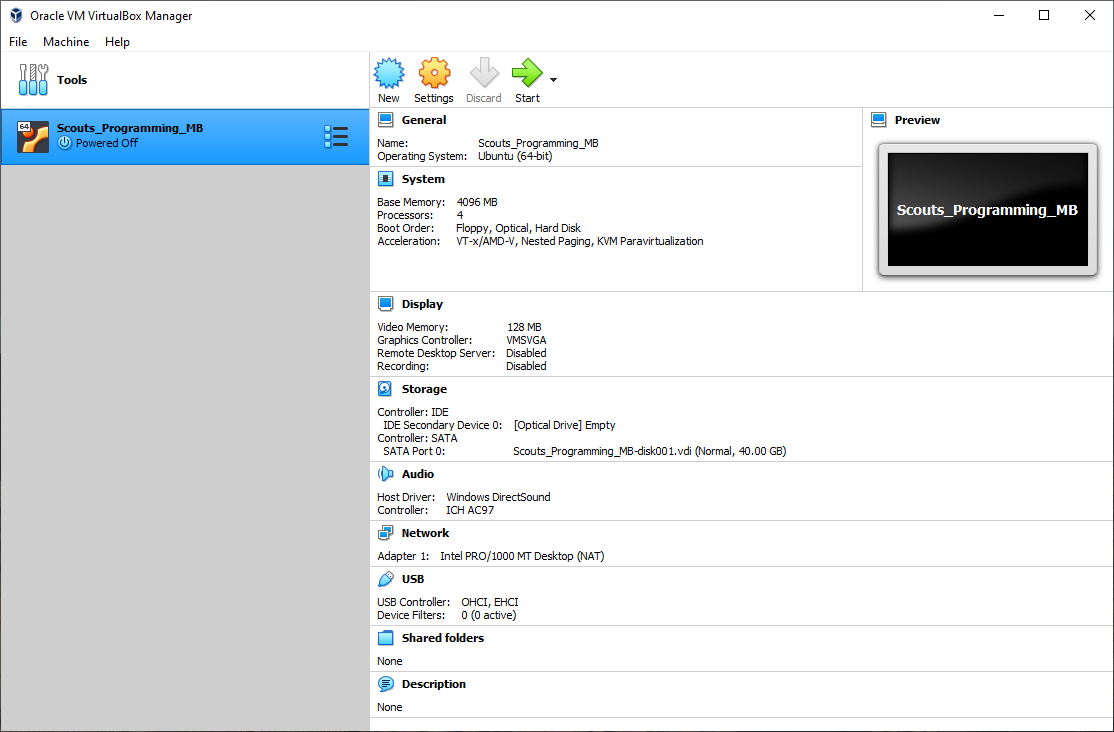
\includegraphics[width=0.8\linewidth]{virtualbox_import_complete.png}
      \caption{VirtualBox Import Complete}
      \label{fig:virtualbox_import_complete}
    \end{figure}
    \FloatBarrier

  \section{Getting Familiar with the VM}
  \label{sec:getting_familiar_with_vm}

    When you first start the VM you will be greeted with a login screen.
    The username and password for the VM can be found below:

    \mdfsetup{
      innertopmargin=12pt,
      linecolor=green!75,
      linewidth=2pt,
      topline=true,
      frametitleaboveskip=\dimexpr-\ht\strutbox\relax,
      nobreak=true
    }

    \vspace{5pt}
    \begin{mdframed}[]
      \textbf{Username:} scoutsbsa

      \textbf{Password:} \texttt{goodturn} 
    \end{mdframed}

    Enter the password and you will be see the home screen.
    In the upper left corner of the screen you should see \autoref{fig:desktop_view}

    \begin{figure}[ht]
      \centering
      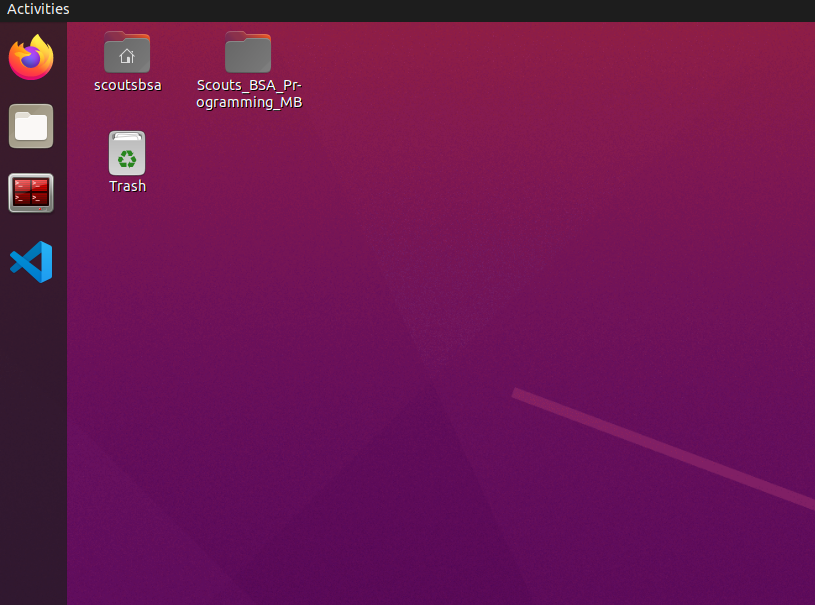
\includegraphics[width=0.8\linewidth]{desktop.png}
      \caption{Desktop View}
      \label{fig:desktop_view}
    \end{figure}

    \FloatBarrier

    There are several icons on this screen.
    The bar on the left contains all of the programs necessary for the projects in this merit badge.
    The top image is the \texttt{FireFox} web-browser (like Google Chrome, Safari, or Internet Explorer).
    One icon down is the file explorer which allows you to see the files on the VM.
    Below the file explorer is the terminal which allows you to compile and execute programs (see \autoref{fig:terminal_icon}).
    Finally, is the the VS Code icon (see \autoref{fig:vs_code_icon}).
    VS Code is a text editor which allows code to be highlighted so it is easier to read.

    \begin{figure}[ht]
      \centering
      \begin{subfigure}{0.4\textwidth}
        \centering
        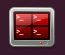
\includegraphics[width=0.5\linewidth]{terminal.png}
        \caption{Terminal Icon}
        \label{fig:terminal_icon}
      \end{subfigure}
      \begin{subfigure}{0.4\textwidth}
        \centering
        
\includegraphics[width=0.5\linewidth]{vs_code.png}
        \caption{VS Code Icon}
        \label{fig:vs_code_icon}
      \end{subfigure}
      \caption{Program Icons}
      \label{fig:program_icons}
    \end{figure}

    \FloatBarrier

    Now click on the terminal open it.
    This will place you in your \textit{home} folder.
    Type the \texttt{ll} command to view a list of all the files and folders in your \textit{home}.

    \begin{figure}[ht]
      \centering
      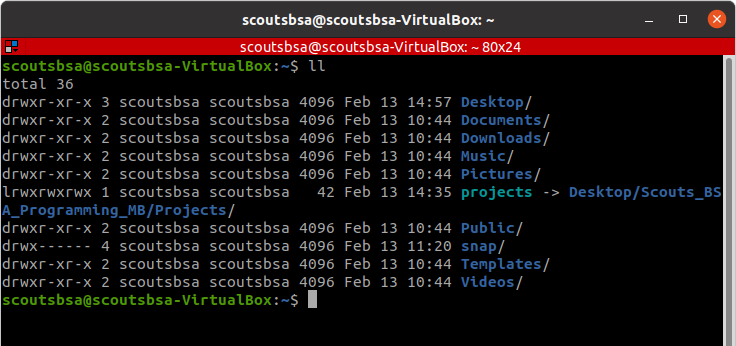
\includegraphics[width=0.8\linewidth]{home_file_list.png}
      \caption{Home Directory File List}
      \label{fig:home_file_list}
    \end{figure}

    \FloatBarrier

    Notice there is a folder called projects.
    This is where all of the files you will need for your projects live.
    To get there in the terminal type \texttt{cd projects}.
    The \texttt{cd} command changes the directory you are in.
    Now find a list of the files in the projects directory.

    \begin{figure}[ht]
      \centering
      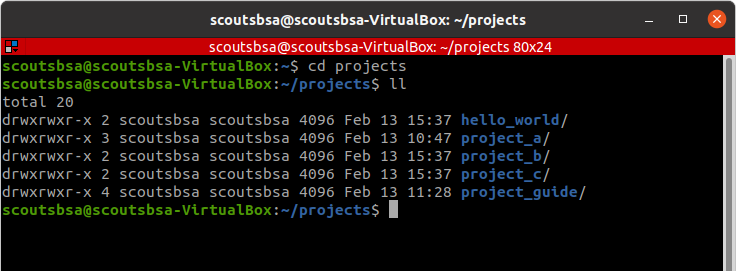
\includegraphics[width=0.8\linewidth]{projects_file_list.png}
      \caption{Project Directory File List}
      \label{fig:proj_file_list}
    \end{figure}

    \FloatBarrier

    Now we want to go into the into the \textit{hello\_world} folder.
    Again use \texttt{cd} to do this.

    Once in the \textit{hello\_world} folder view the two files using \texttt{ll}.
    Notice a file called \textit{Makefile}.
    This is the file which controls how all of your projects are run.
    Use the command \texttt{make} to view what it does in this folder.

    \begin{figure}[ht]
      \centering
      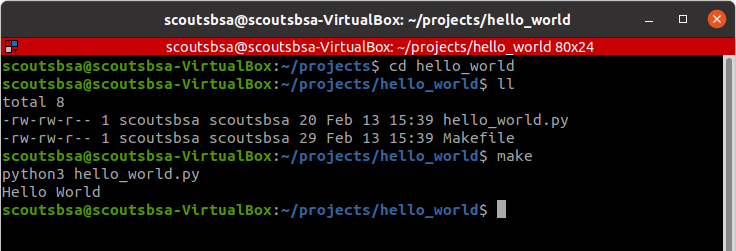
\includegraphics[width=0.8\linewidth]{hello_world.png}
      \caption{Project Directory File List}
      \label{fig:hello_world_example}
    \end{figure}

    \FloatBarrier

    Now that you've seen how we are going to run our projects let's explore how we are going
      to change the code.
    Open the VS Code window by clicking on the VS Code icon on the left.
    The left hand side should contain a list of files and folders.
    At the top of this section the folder name which you are currently looking at 
      should be displayed.
    VS Code should have automatically opened to the \texttt{projects} folder.
    If not use \textit{File $\rightarrow$ Open Folder} to open the projects folder in your home directory.

    Now click the hello world folder on the left-hand bar.
    You should see the same two files we saw in the terminal.
    Click \texttt{hello\_world.py} to open the file.
    This file is extremely simple, so for now just change the "Hello World" message to another message of your choosing.
    Then rerun make in the terminal.
    You should now see your message displayed!

  \section{Next Steps}
  \label{sec:next_steps}

    Now you should be ready to go!
    Head on over to the \nameref{chap:project_a} chapter to get started.

    If you've had any troubles in this section let your councilor know before moving on.